\subsection{Serving \& Security}
Our infrastructure's security is handled on several layers by a variety of services striving to offer access on data and visualisations to the users and to let the developers maintain and upgrade the system while providing extensive security on the data and protection from unauthorised access.

\begin{figure}[h]
	\centering
	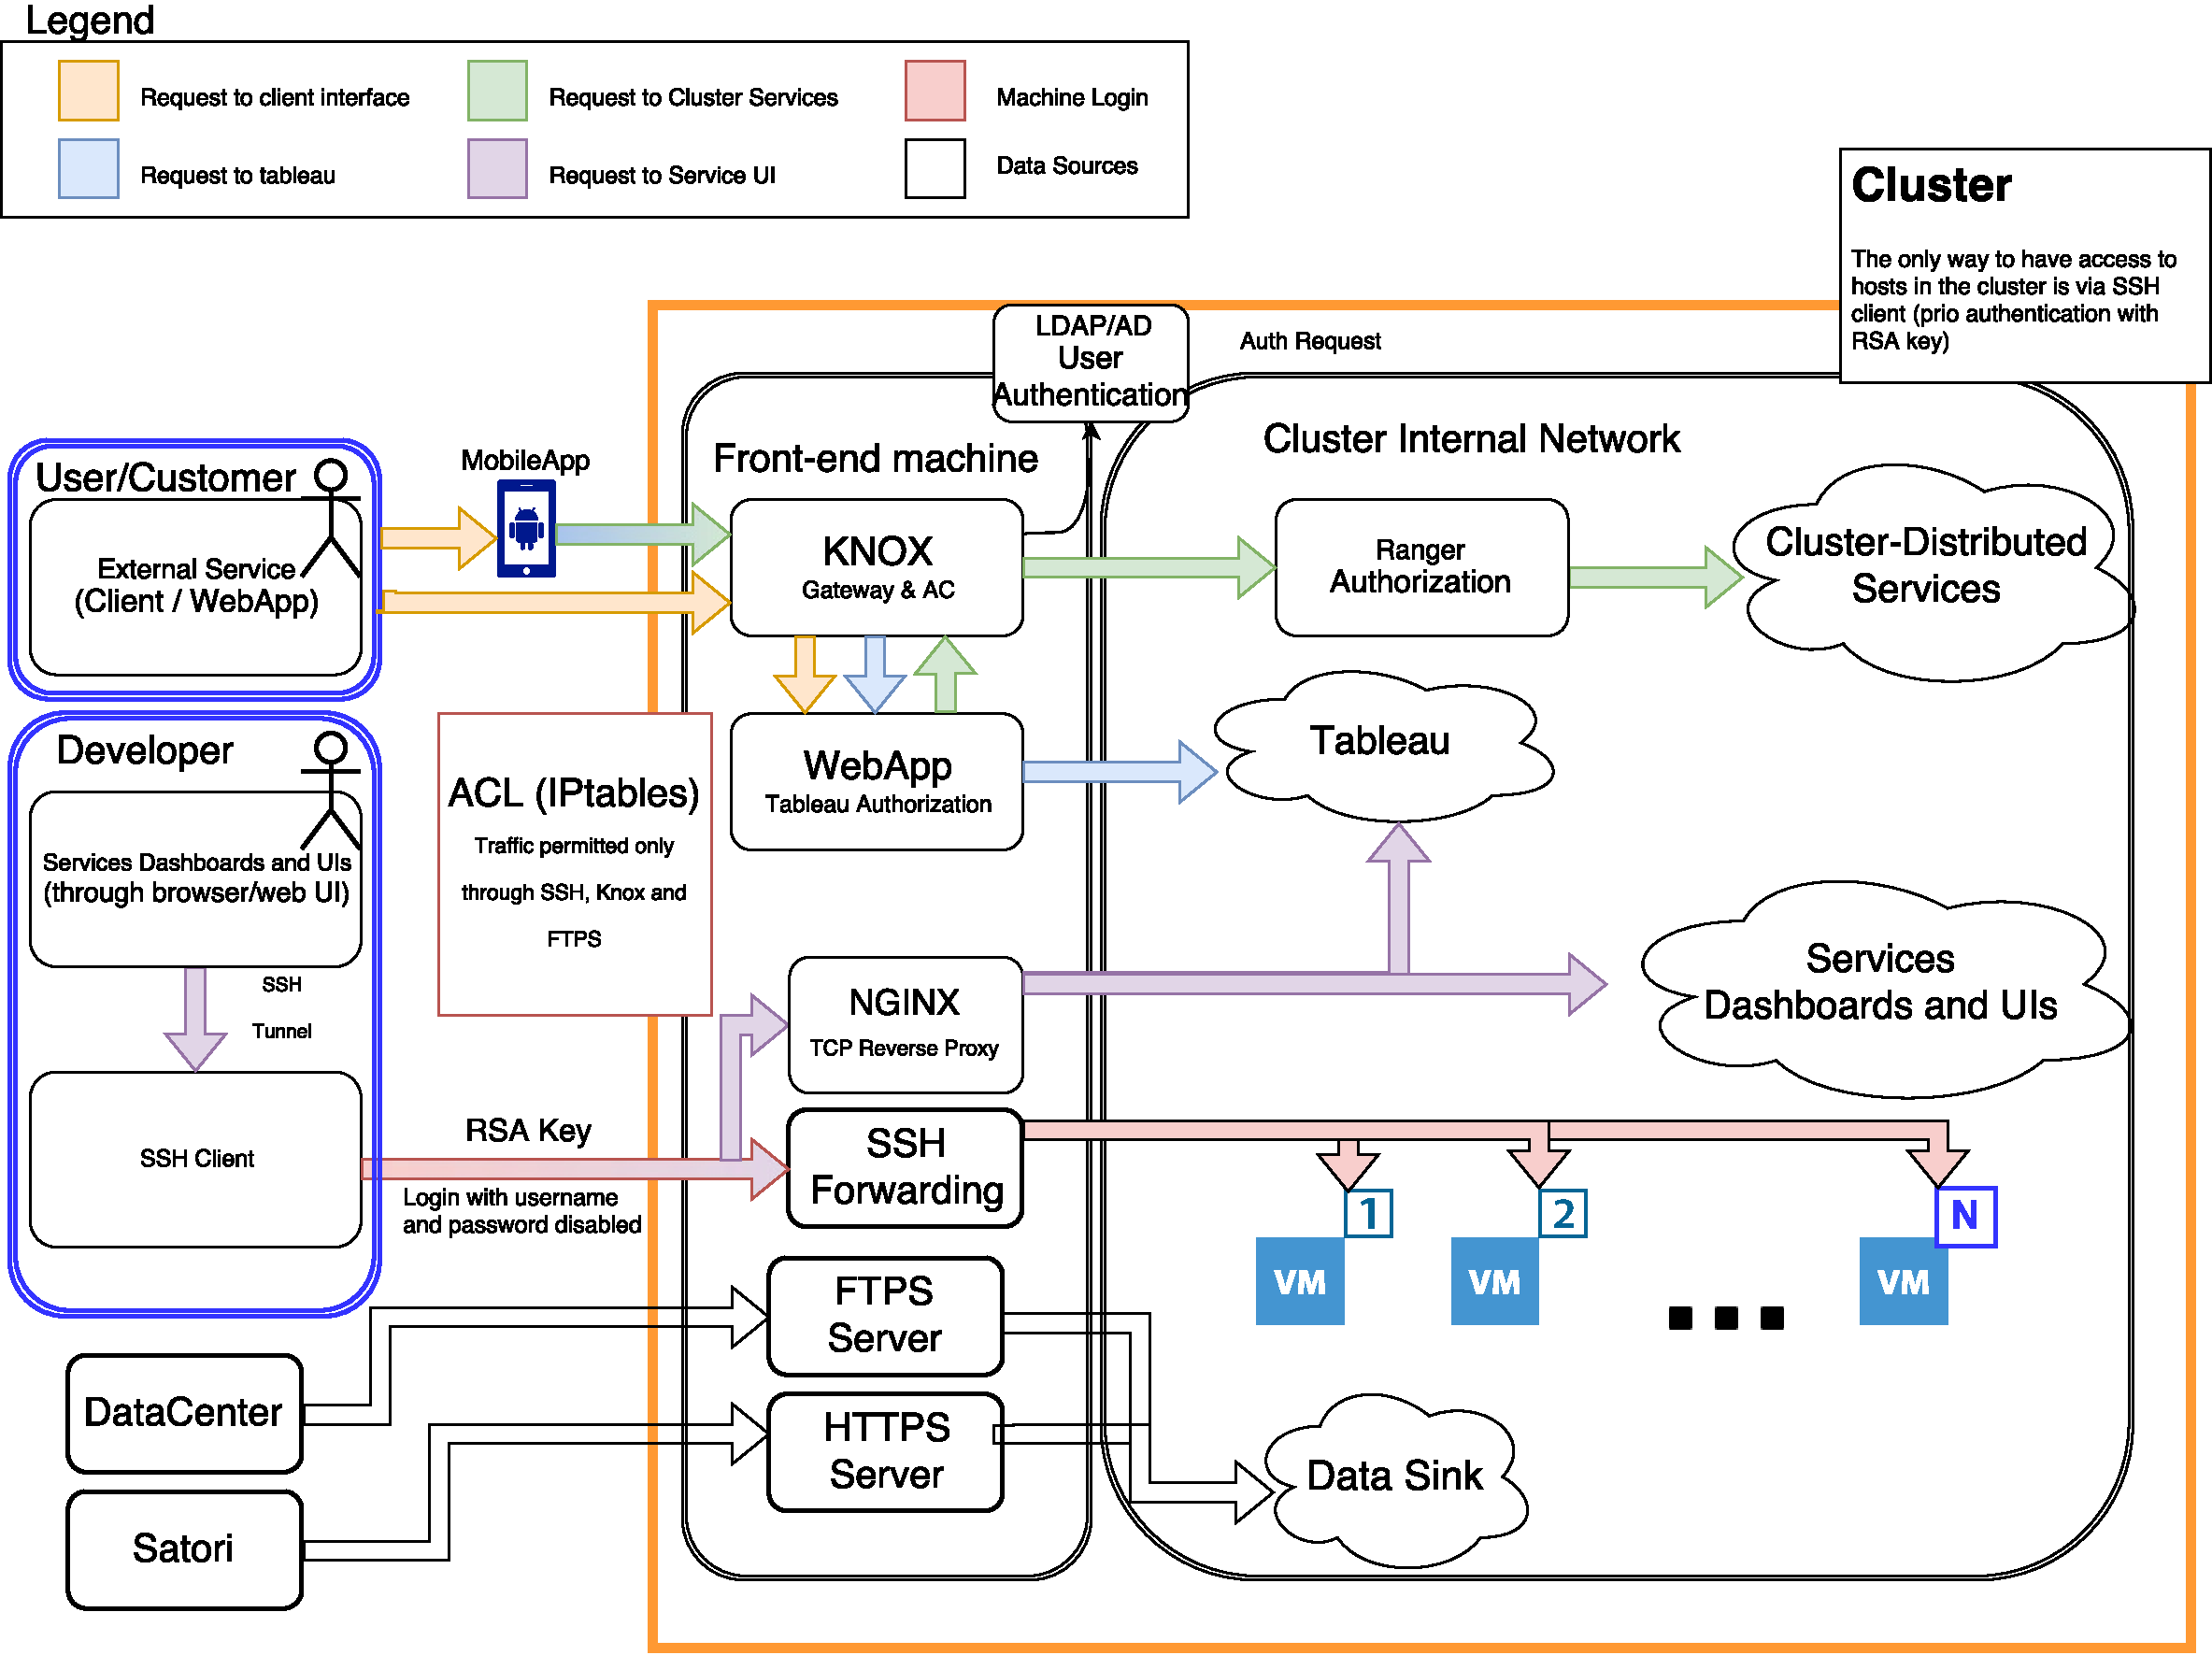
\includegraphics[scale=0.3]{Figures/SecurityStructureDiagram}
	\decoRule
	\caption[Security Structure Diagram]{A diagram to represent our Security Structure}
	\label{fig:SecurityStructureDiagram}
\end{figure}

We have structured the Security and Serving architecture through two main abstractions: the \textbf{cluster} and the \textbf{flows}.
\subsubsection{Cluster}
The \textbf{cluster} is our whole Big Data Infrastructure comprised of several nodes which for our purposes are divided as such:
\begin{itemize}
	\item One (or two in High Availability) Domain Controller, which handles user creation, update and authentication.
	\item One (or two in High Availability) Front End node, which manages access to the cluster's services and data.
	\item Several Inner Cluster nodes, the machines on which visualising, processing and storing is actually done.
\end{itemize}

\paragraph{Domain Controller}
The Domain Controller is not accessible from outside the cluster and can communicate freely with the Front End and the Inner Cluster Nodes.\\
It hosts \textbf{Active Directory}, a directory service by Microsoft comprised of several components for domain and security management such as LDAP, Kerberos, and DNS.\\ \\
As a directory service, the Active Directory instance consists of a database containing an hierarchy of objects, objects are a very high abstraction that can represent a variety of things, but for our purposes can either be Users or Groups; Groups contain one or more Users and Users may be part of one or more Groups. \\Users are identified by a username and a strong password, thus the Domain Controller can authenticate an Agent thanks to this information. \\
Through LDAP, authorised Users can access and modify Objects in the Active Directory. Each authentication, whether failed or successful is logged.\\ \\
We have defined two groups: \texttt{cluster\_users} and \texttt{cluster\_operators}, the meaning of which is further specified down the line by each layer of protection.

\paragraph{Front End}
The Front End node is the only machine accessible from outside the cluster and can communicate with the Domain Controller and the Inner Cluster nodes. \\
Access to the Front End from outside is possible through a selected number of ports and only with secure protocols (HTTPS, FTPS and SSH), this is obtained with the use of ACLs, implemented on CentOS through iptables. The Front End features Apache Knox and Nginx to route requests to the right services and stores RSA private keys of all the Inner Cluster nodes plus a public one for each developer's own private key, so that passwordless SSH connections can be established from developers' machines to Front End and from Front End to Inner Cluster nodes. \\
\\
Nginx is a HTTP and HTTPS reverse proxy that also supports TCP reverse proxying and can be used to route whatever HTTP request or TCP connection from the Front End machine to the proper Inner Cluster node's service. \\
\\
Apache Knox also serves as a reverse proxy, this time specifically for Hadoop cluster's services requiring authentication and authorisation. Its topology is implemented so that an authorised Active Directory user called Knox.domain, through LDAP, can ask for authentication on an incoming request's sender and access to lists of Users and Groups.\\ If the user is authenticated, Knox can then grant access to the request, thanks to the information on Users and Groups, to the target service and route it accordingly or deny it. \\ Outcoming requests are bundled with the authenticated username, so that inside the Inner Cluster nodes other services can use that information securely. Requests at this stage are logged whether denied or accepted, along the name of the alleged requester in order to be investigated in case of failures or attempted breaches.\\ \\
The topology is set so that all our custom services for access to MongoDB and Hive are available to all users belonging to the cluster\_users or cluster\_operators group, while the standard Hadoop services are available only to those in the latter.
\\
\\
The Front End machine also hosts programs for data ingestion, an FTPS server and a NodeJS application that serves the WebApp.

\paragraph{Inner Cluster Nodes}

All the other nodes in the Cluster are considered Inner nodes as they are barred from outside and can only communicate with the Domain Controller and the Front End. \\
These machines hold all processing services, databases and visualisation tools plus the interfaces to access their resources. Here, requests incoming from the Front End have been already authenticated and given access, but each service can enact additional policies on those, to add a layer of security and to protect from mistakes (i.e. DROP DATABASE). \\ \\
While each service might manage its own policies, most Hadoop applications delegate this burden to Apache Ranger: Ranger, thanks to its Usersync agent synchronises its list of Users and Groups with the Active Directory's one, so that further authorisation policies can be defined on the same cluster\_users and cluster\_operators seen before. \\ \\
 Thus we have decided to give users in cluster\_users clearance for the use of SELECT on our Air-Traffic database, while deletions are forbidden to them; on the other end, users in cluster\_operators are also able to update and delete records.
\\ At this level, requests are logged again, to log failed authorisations and to assign actions' responsibilities to the appropriate users.

\subsubsection{Flow}
We define the flow, in the context of the security of our system, as the path requests and responses travel from a class of external Actors to the cluster and back.
\\ \\
In general, the flow starts from an Actor outside the cluster sending a request (i.e. A User through a MobileApp), the request is received by the Front End Node, accepted or denied; accepted requests are then forwarded and routed to the target Inner Node's service which handles the request and generates a response accordingly, the response is then set back following the same path backwards to the Actor.
\\ \\
We have distinguished three different flows, each pertaining to a different Actor:
\paragraph{User}
A user, which is a person or agent requesting access to our stored data, can query our databases and view visualisations built upon stored data service through a WebApp or a Mobile App.\\
Queries are sent to our custom REST APIs to Knox on the Front End machine; the user, who must be present in Active Directory and be part of cluster\_users, is authenticated and authorised to proceed with its request, this request now routed to the Inner Cluster is received by our REST servers, parsed into queries and sent to the appropriate database with the user's credentials, the query is received by MongoDB security or Apache Ranger for Hive, whatever the recipient, its policies are enforced on the request; the result of the query is then sent back to the REST server which encapsulate it and send it back as a response to the user.
\\ \\
Visualisations are requested to the WebApp from outside the cluster, the WebApp requires a login for authentication and then authorises the user following its own policies, as a Tableau user or operator, the WebApp then requests tokens to be consumed watching visualisations on behalf of the user and then responds with a HTML page embedding the visualisations and tokens. This method prevents the need of having to authenticate the same users multiple times.
\paragraph{Developer}
While able to access the cluster as clients, the developers can also connect to the Front End through an SSH client provided they have the Front End private key, as username and password are disabled, while connected they can further their connections to all nodes to access the local file system. What's more, through tunnelling, several TCP connections can be forwarded through the SSH connection from the developer localhost to the Front End machine; there Nginx routes Front End local connections to several clusters' machines, providing a safe passage from the developer's machine to the required Dashboard or User Interface.
\paragraph{Data Source}
Lastly Data Sources must be able to send data to our secured clusters to be stored on the databases, in order to do that two options are available: an application on the Front End can pull data constantly on an endpoint (for example through HTTPS) or the providers can push data on a server on the Front End (for example through FTPS), then another application is responsible to transfer newly acquired data from the Front End to the Inner Cluster Nodes
\pagebreak